\chapter{}
\begin{center}
	\Huge\textbf{premier chapter}	
\end{center}

\section{Introduction}
L’une des récentes avancées dans la micro électronique et des technologies sans-fil qui confortent la présence de l’informatique et de l’électronique au cœur du monde réel ont permis de développer des capteurs de petite taille. Ces  micro-capteurs sont dotés d’une capacités de traitement permettant de collecter et de transmettre des données environnementales d'une manière autonome.Les réseaux de capteurs sans fil ou WSNs(Wireless Sensor Networks) sont constitués d’un ensemble de capteurs sans fil s’auto organisant pour acquérir des données de leur environnement immédiat, de les traiter et de les communiquer.
Dans ce premier chapitre, nous présenterons un ensemble de généralités sur les réseaux de capteurs, notamment sur leur architecture et leurs domaines d’applications.\\

\section{Un réseau de capteur sans-fil}
un réseau de capteur sans fil est un type spécial de réseau ad-hoc où la plupart de ces nœuds sont des micro-capteurs dispersés dans une zone géographique appelée zone de captage. La position de ces nœuds n’est pas obligatoirement déterminée, ils utilisent une communication sans fil pour acheminer les données captées avec un routage multi sauts vers un nœud collecteur appelé nœud puits(Sink). Ces capteurs comme ils ont été décrit au paravent  sont des diapositifs de taille extrêmement réduite avec des sources limitées, autonome, capable de traiter et transmettre les informations.

\begin{center}
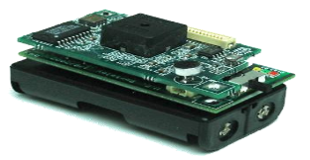
\includegraphics[width=7cm,height=3.7cm]{Chap1/chap1.png}
\end{center}


Les réseaux de capteurs utilisent un très grand nombre de ces capteurs, pour former un réseau sans infrastructure établie. Chaque capteur relayant l'information sur sa propre zone de couverture, le réseau se trouve entièrement couvert.

\begin{center}
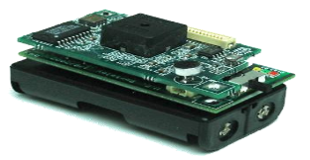
\includegraphics[width=7cm,height=3.7cm]{Chap1/chap1.png}
\end{center}

